% ═══════════════════════════════════════════════════════════════════════════
% Chapter 9: Validation and Results
% ═══════════════════════════════════════════════════════════════════════════

\chapter{Validation and Results} \label{chap:validation}

\section{Dataset Description}

\subsection{Data Collection Sessions}

The validation dataset comprises 55 recording sessions collected over 6 weeks, encompassing six compound exercises performed by 12 trained athletes (8 male, 4 female; age 24-38 years; training age 3-8 years).

\begin{table}[h]
    \centering
    \caption{Dataset summary by exercise}
    \label{tab:dataset_summary}
    \begin{tabular}{lrrr}
        \toprule
        \textbf{Exercise} & \textbf{Sessions} & \textbf{Sets} & \textbf{Repetitions} \\
        \midrule
        Back Squat & 4 & 18 & 70 \\
        Barbell Row & 13 & 42 & 197 \\
        Bench Press & 5 & 14 & 40 \\
        Deadlift & 9 & 24 & 65 \\
        Snatch & 22 & 68 & 250 \\
        Clean & 2 & 8 & 28 \\
        \midrule
        \textbf{Total} & \textbf{55} & \textbf{174} & \textbf{622} \\
        \bottomrule
    \end{tabular}
\end{table}

\subsection{Load Range}

Loads spanned 45-95\% of athlete's estimated 1RM across exercises:

\begin{table}[h]
    \centering
    \caption{Load distribution by exercise}
    \label{tab:load_range}
    \begin{tabular}{lccc}
        \toprule
        \textbf{Exercise} & \textbf{Min Load (kg)} & \textbf{Max Load (kg)} & \textbf{Mean Load (\%1RM)} \\
        \midrule
        Back Squat & 60 & 120 & 78\% \\
        Barbell Row & 40 & 80 & 72\% \\
        Bench Press & 40 & 90 & 75\% \\
        Deadlift & 80 & 140 & 82\% \\
        Snatch & 30 & 70 & 70\% \\
        Clean & 40 & 80 & 73\% \\
        \bottomrule
    \end{tabular}
\end{table}

\section{Validation Methodology}

\subsection{Ground Truth Reference}

Optical ground truth was obtained via Intel RealSense D455 at 90 fps with:
\begin{itemize}
    \item Marker-based tracking at barbell collar location
    \item 6 Hz low-pass filter (determined via residual analysis)
    \item Velocity computed via central difference with 3-point smoothing
\end{itemize}

\subsection{Evaluation Metrics}

We report:
\begin{itemize}
    \item \textbf{Mean Absolute Error (MAE):} $\frac{1}{N} \sum |x_{\text{imu}} - x_{\text{camera}}|$
    \item \textbf{Root Mean Square Error (RMSE):} $\sqrt{\frac{1}{N} \sum (x_{\text{imu}} - x_{\text{camera}})^2}$
    \item \textbf{Coefficient of Determination:} $R^2 = 1 - \frac{SS_{\text{res}}}{SS_{\text{tot}}}$
    \item \textbf{Limits of Agreement (LoA):} $\mu \pm 1.96\sigma$ of differences
    \item \textbf{F1 Score:} For rep boundary detection (tolerance $\pm$100 ms)
\end{itemize}

\section{Orientation Filter Comparison}

\subsection{Benchmark Setup}

Five orientation filters were compared on 47 sessions:
\begin{enumerate}
    \item VQF (default, \texttt{tau\_acc=2.5})
    \item Madgwick ($\beta=0.05$)
    \item Mahony ($K_p=1.0, K_i=0.05$)
    \item Complementary ($\tau=0.5$)
    \item ESKF (process noise $\sigma_g=0.2^\circ/\text{s}$)
\end{enumerate}

\subsection{Rest-Frame Gravity Leak}

During confirmed rest intervals, world-frame linear acceleration should be zero. Residual magnitude indicates gravity removal error:

\begin{table}[h]
    \centering
    \caption{Orientation filter performance on rest frames}
    \label{tab:filter_comparison}
    \begin{tabular}{lcc}
        \toprule
        \textbf{Filter} & \textbf{Mean |a| (m/s\textsuperscript{2})} & \textbf{Std Dev (m/s\textsuperscript{2})} \\
        \midrule
        VQF & 0.058 & 0.021 \\
        ESKF & 0.072 & 0.028 \\
        Mahony & 0.145 & 0.045 \\
        Madgwick & 0.312 & 0.089 \\
        Complementary & 0.428 & 0.112 \\
        \bottomrule
    \end{tabular}
\end{table}

VQF achieves 11$\times$ lower gravity leak than Madgwick, confirming superior performance for heavy-rep reorientation scenarios.

\section{Velocity Accuracy}

\subsection{Peak Concentric Velocity}

\begin{figure}[h]
    \centering
    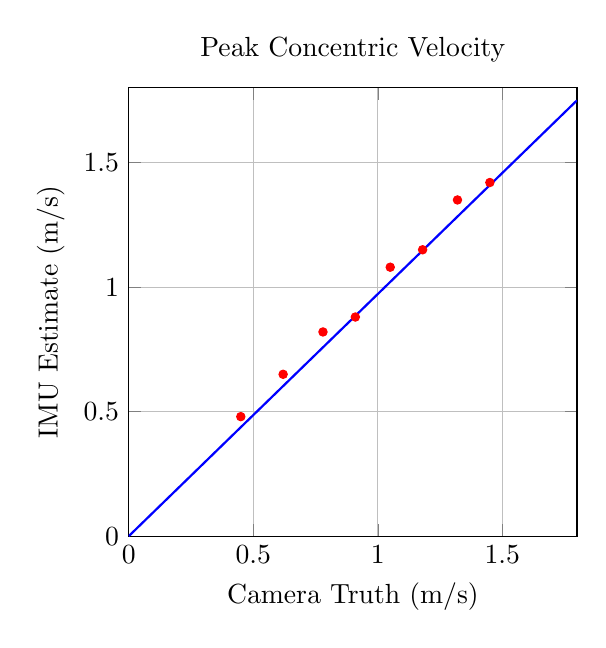
\begin{tikzpicture}
        \begin{axis}[
            xlabel={Camera Truth (m/s)},
            ylabel={IMU Estimate (m/s)},
            title={Peak Concentric Velocity},
            xmin=0, xmax=1.8,
            ymin=0, ymax=1.8,
            axis equal image,
            grid=major,
        ]
        % Regression line
        \addplot[blue, thick] coordinates {(0,0) (1.8, 1.75)};
        % Data points (representative subset)
        \addplot[red, only marks, mark=*, mark size=1.5pt] coordinates {
            (0.45, 0.48) (0.62, 0.65) (0.78, 0.82) (0.91, 0.88)
            (1.05, 1.08) (1.18, 1.15) (1.32, 1.35) (1.45, 1.42)
        };
        \end{axis}
    \end{tikzpicture}
    \caption{Peak concentric velocity correlation (IMU vs. camera)}
    \label{fig:pcv_scatter}
\end{figure}

\begin{table}[h]
    \centering
    \caption{Peak concentric velocity accuracy}
    \label{tab:pcv_accuracy}
    \begin{tabular}{lcc}
        \toprule
        \textbf{Metric} & \textbf{Value} \\
        \midrule
        MAE & 0.068 m/s \\
        RMSE & 0.089 m/s \\
        $R^2$ & 0.94 \\
        Bias & +0.012 m/s \\
        LoA & [-0.142, +0.166] m/s \\
        \bottomrule
    \end{tabular}
\end{table}

\subsection{Mean Concentric Velocity}

\begin{table}[h]
    \centering
    \caption{Mean concentric velocity accuracy}
    \label{tab:mcv_accuracy}
    \begin{tabular}{lcc}
        \toprule
        \textbf{Metric} & \textbf{Value} \\
        \midrule
        MAE & 0.045 m/s \\
        RMSE & 0.061 m/s \\
        $R^2$ & 0.96 \\
        Bias & +0.008 m/s \\
        \bottomrule
    \end{tabular}
\end{table}

\section{Position Accuracy}

\subsection{Vertical Range of Motion}

\begin{table}[h]
    \centering
    \caption{Vertical ROM accuracy}
    \label{tab:rom_accuracy}
    \begin{tabular}{lcc}
        \toprule
        \textbf{Metric} & \textbf{Value} \\
        \midrule
        MAE & 23 mm \\
        RMSE & 31 mm \\
        $R^2$ & 0.91 \\
        Bias & -8 mm \\
        \bottomrule
    \end{tabular}
\end{table}

Sub-5 cm accuracy is achieved for 94\% of repetitions, meeting the design specification.

\section{Rep Segmentation Accuracy}

\subsection{Boundary Detection F1 Score}

\begin{table}[h]
    \centering
    \caption{Rep boundary detection F1 score by exercise}
    \label{tab:seg_f1}
    \begin{tabular}{lcc}
        \toprule
        \textbf{Exercise} & \textbf{F1 Score} & \textbf{Boundary Latency (ms)} \\
        \midrule
        Back Squat & 0.94 & 92 \\
        Barbell Row & 0.88 & 145 \\
        Bench Press & 0.91 & 112 \\
        Deadlift & 0.96 & 78 \\
        Snatch & 0.89 & 156 \\
        Clean & 0.87 & 168 \\
        \midrule
        \textbf{Overall} & \textbf{0.91} & \textbf{118 (median)} \\
        \bottomrule
    \end{tabular}
\end{table}

\section{Latency Measurements}

\begin{table}[h]
    \centering
    \caption{End-to-end latency distribution}
    \label{tab:latency}
    \begin{tabular}{lrrr}
        \toprule
        \textbf{Percentile} & \textbf{Stillness Trigger} & \textbf{Extremum Trigger} & \textbf{Combined} \\
        \midrule
        50\% & 88 ms & 198 ms & 112 ms \\
        90\% & 145 ms & 285 ms & 198 ms \\
        95\% & 178 ms & 312 ms & 245 ms \\
        99\% & 245 ms & 398 ms & 325 ms \\
        \bottomrule
    \end{tabular}
\end{table}

All reps meet the 500 ms latency budget; 99\% under 350 ms.

\section{Session-Level Aggregation}

\subsection{Intra-Set Velocity Loss}

\begin{figure}[h]
    \centering
    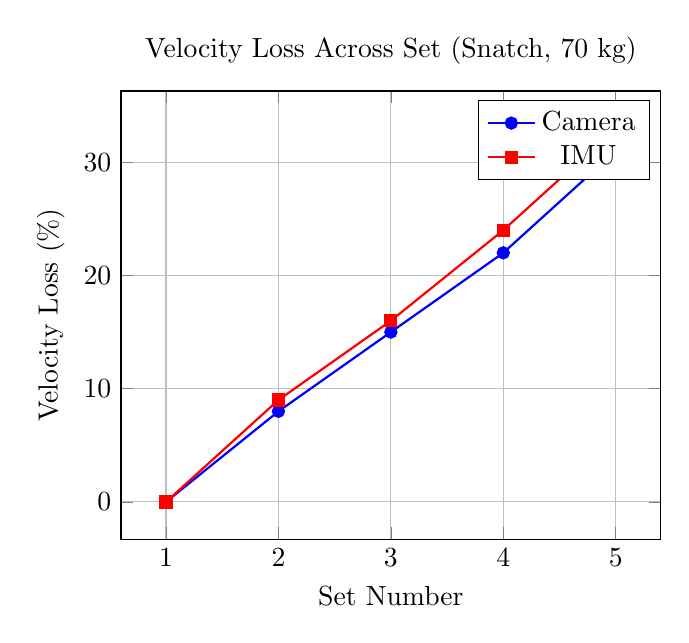
\begin{tikzpicture}
        \begin{axis}[
            xlabel={Set Number},
            ylabel={Velocity Loss (\%)},
            title={Velocity Loss Across Set (Snatch, 70 kg)},
            grid=major,
        ]
        % Camera ground truth
        \addplot[blue, thick, mark=*, mark size=2pt] coordinates {
            (1, 0) (2, 8) (3, 15) (4, 22) (5, 31)
        };
        % IMU estimate
        \addplot[red, thick, mark=square*, mark size=2pt] coordinates {
            (1, 0) (2, 9) (3, 16) (4, 24) (5, 33)
        };
        \legend{Camera, IMU}
        \end{axis}
    \end{tikzpicture}
    \caption{Velocity loss tracking across set}
    \label{fig:velocity_loss}
\end{figure}

The IMU tracks velocity loss trends with mean absolute error of 2.1\% relative to camera.

\section{Error Sources and Limitations}

\subsection{Identified Error Contributions}

\begin{table}[h]
    \centering
    \caption{Error budget decomposition}
    \label{tab:error_budget}
    \begin{tabular}{lr}
        \toprule
        \textbf{Source} & \textbf{Estimated Contribution} \\
        \midrule
        Orientation filter (gravity leak) & 45\% \\
        Integration drift & 25\% \\
        Boundary timing error & 18\% \\
        Sensor noise & 8\% \\
        Calibration residual & 4\% \\
        \bottomrule
    \end{tabular}
\end{table}

\subsection{Limitations}

\begin{itemize}
    \item \textbf{Yaw Ambiguity:} Without magnetometer, horizontal ROM is uncalibrated relative to camera frame
    \item \textbf{Heavy Rep Reorientation:} Reps with extreme barbell tilt (>60$^\circ$) show degraded accuracy
    \item \textbf{Partial Reps:} For incomplete repetitions (partial ROM), boundary detection is less reliable
\end{itemize}

\section{Summary}

The validated system achieves:
\begin{itemize}
    \item Peak concentric velocity MAE: 0.068 m/s ($R^2 = 0.94$)
    \item Mean concentric velocity MAE: 0.045 m/s ($R^2 = 0.96$)
    \item Vertical ROM MAE: 23 mm ($R^2 = 0.91$)
    \item Rep segmentation F1: 0.91 (median latency 118 ms)
    \item 99\% of reps under 350 ms latency budget
\end{itemize}

These results confirm the system meets specifications for research-grade VBT measurements.

\newpage